\chapter{Results and Future work}
\label{ch:results}

This chapter presents the results of the realizations conducted in the previous chapter. It proposes an analysis of the next steps that someone in the future could take to improve the system.

\section{Objectives fullfilement}
\subsection{Recording system}

Once we installed the recording system on the HEIA-FR building, it allowed us to record the street at any time and generate large amounts of data. The system was reliable, always available, and thanks to the script to run it, it was also easy to use.

\paragraph*{Problems encountered}

We first tried streaming the data directly from the raspberry pi to the storage server with the Real-time Transport Protocol (RTP) \footnote{\url{https://fr.wikipedia.org/wiki/Real-time\_Transport\_Protocol}}. By default, the RTP protocol did not encrypt the streamed data. The \textit{ffmpeg} encoding buffer was regularly full, which caused the loss of some frames and some artifacts in the audio, and the streaming technique gave us a bad image quality due to the real-time encoding of the video.

We solved all these problems by using the SFTP protocol. We solved the image quality by mounting the storage server's folder on the raspberry pi as a network driver. Since ffmpeg no longer used the RTP, it could take his time to encode the video in good quality and save it. The SFTP use also solved the buffer issue. Finally, the SFTP protocol allowed us to encrypt the data since it's a secure protocol by default. An example of the difference between the two method's quality can be seen in the figure \ref{fig:streaming}.

\begin{figure}[H]
    \centering
    \subfloat[Frame quality with RTP]{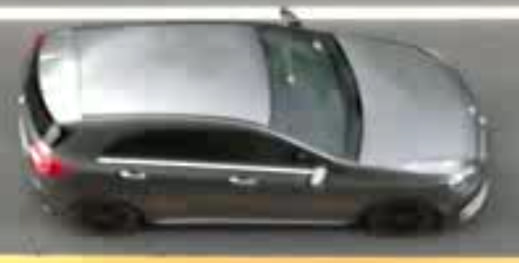
\includegraphics[width=0.45\textwidth]{images/streaming_rtp.png}\label{fig:streaming_rtp}}
    \qquad
    \subfloat[Frame quality with SFTP]{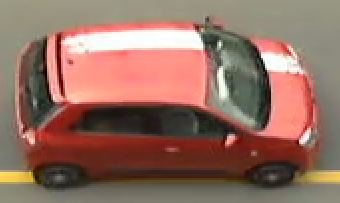
\includegraphics[width=0.45\textwidth]{images/streaming_sftp.png}\label{fig:streaming_sftp}}
    \caption{Comparison of the frame quality between the two streaming methods}
    \label{fig:streaming}
\end{figure}

Even if the quality difference is not considerable, using the SFTP protocol was a nice side effect of changing the streaming method.

\section{Definition of the baseline}

With the analysis and design parts of the report (section \ref{sec:baseline_analysis} and \ref{sec:baseline_design}), we defined the baseline as a set of steps to follow to achieve the goal of this project. The baseline described in this report is accurate and complete enough to be followed by someone else in the future. The definition achieves the first objective of creating a baseline in section \ref{intro:objective1}. 

\section{Real-life dataset}

With the recording system in place, we built a dataset for this project comprising 2028 dual-channel audio and video files of 2 seconds classified into four classes. The realization of this dataset achieves the goal defined in section \ref{intro:objective2} of having a dataset that follows the baseline to train our model. The dataset is complete and follows the baseline. It is also large enough to train a model with it. The dataset's creation solves the problem of the lack of a dataset for this project. We can consider the objective defined in section \ref{intro:objective2} as achieved.

Although the dataset is created and follows the baseline, it is questioned in the next section ()\ref{sec:neural_network_results}).

\section{Neural Network model results}
\label{sec:neural_network_results}

We trained the neural network multiple times and tested it on the test set. The results were not as good as expected. The model was not able to classify the \textit{no\_car} and the \textit{multiple\_cars} classes very well. The model could not accurately classify the \textit{right\_to\_left} and \textit{left\_to\_right} classes. We trained the model with different percentages of the dataset in the train set. First with 60\%, then with 70\%, and finally with 80\%.
The results are presented in the table \ref{tab:neural_network_results}.

\begin{figure}[H]
    \centering
    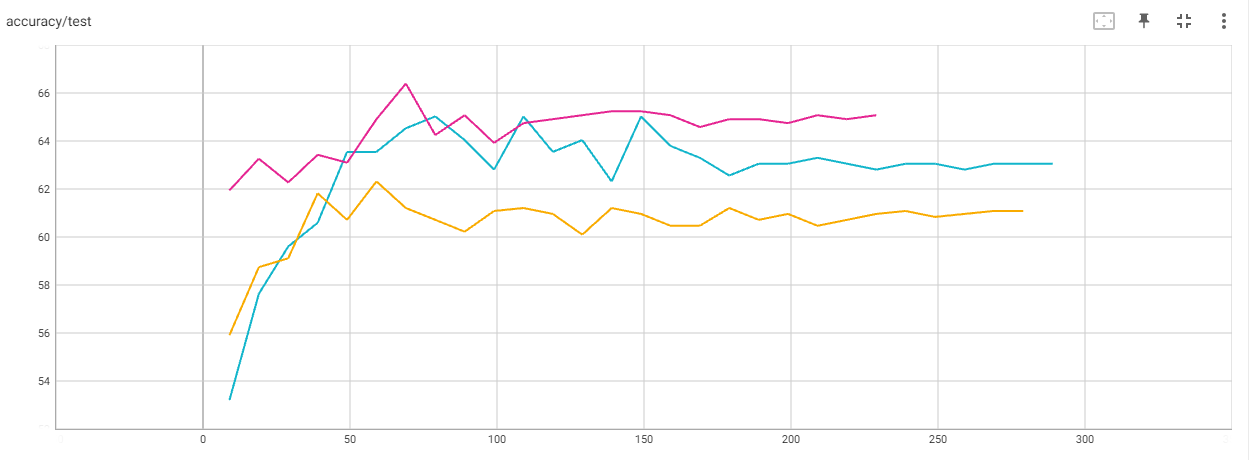
\includegraphics[width=0.8\textwidth]{images/accuracy_test.png}
    \caption{Accuracy of the neural network model for each train set proportion. Orange is 60\%, purple is 70\%, and pink is 80\%}
    \label{ftab:neural_network_results}
\end{figure}

We can see that the model trained with 70\% of the dataset in the train set is the one that has the best accuracy. It might mean that using the 80\% dataset in the train set is too much, and the model overfits the data. If we look at the loss graph (figure \ref{fig:loss_test}), we can see that the model trained with 60\% of the dataset in the train set has a higher loss than the two others. 

\begin{figure}[H]
    \centering
    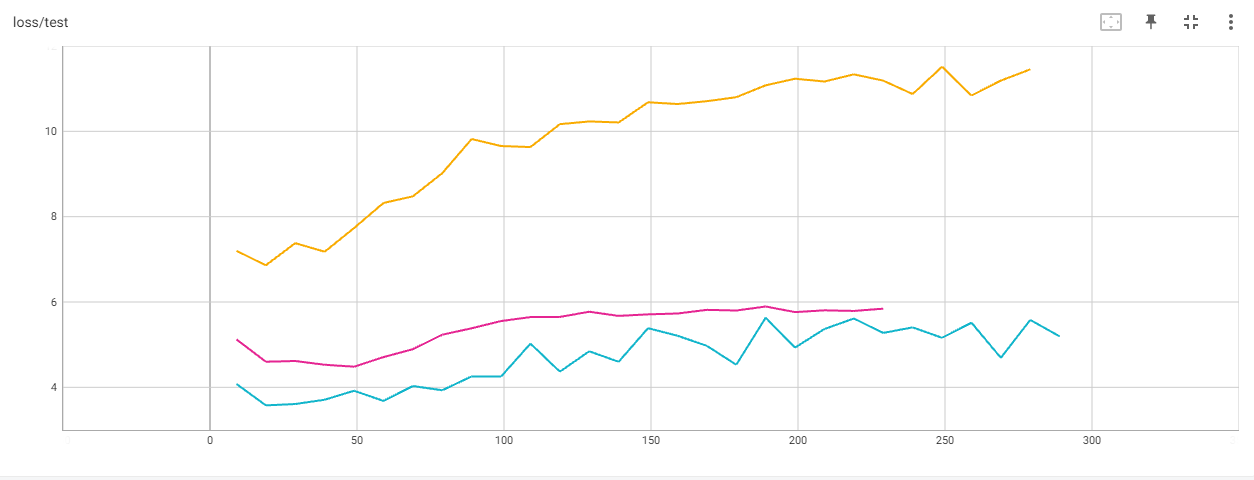
\includegraphics[width=0.8\textwidth]{images/loss_test.png}
    \caption{Loss of the neural network model each train set proportion. Orange is 60\%, purple is 70\%, and pink is 80\%}
    \label{fig:loss_test}
\end{figure}

The accuracy and loss of the models are presented in the next table. We added the runs with the 40\%, 50\%, and 90\% of the dataset in the train set to the table \ref{tab:neural_network_results} to show that the model's accuracy and loss are not better with these percentages.

\begin{table}[H]
    \centering
    \begin{tabular}{|l|l|l|l|}
    \hline
    \textbf{Train set} & \textbf{Test set} & \textbf{Accuracy} & \textbf{Loss} \\ \hline
    40\%               & 60\%              & 0.6071              & 21.32         \\ \hline
    50\%               & 50\%              & 0.612               & 9.55          \\ \hline
    60\%               & 40\%              & 0.6305              & 11.45         \\ \hline
    70\%               & 30\%              & 0.6507              & 5,844         \\ \hline
    80\%               & 20\%              & 0.6108              & 5.19          \\ \hline
    90\%               & 10\%              & 0.5095              & 6.33          \\ \hline
    \end{tabular}
    \caption{Accuracy and loss of the neural network model for each train set percentage}
    \label{tab:neural_network_results}
\end{table}

We can see in the table \ref{tab:neural_network_results} that the model trained with 70\% of the dataset in the train set has the best accuracy and loss. We can also see that the model trained with 90\% of the dataset in the train set has the worst accuracy and loss. We can see that the loss with the small train set is big, so the model cannot generalize well.

\paragraph{Problem encountered}

We might have a case of overfitting. To solve this problem, we have multiple possibilities.

\begin{itemize}
    \item We can do an early stopping of the training. We can stop the training when the loss on the test set starts to increase. 
    \item We also can construct a bigger dataset. Since we could train the model on more data, it would generalize better and be less likely to overfit.
\end{itemize}

\paragraph{Solution}




\subsection{Dataset quality}




\subsection{Dataset Augmentation}
\label{sec:augmentation_results}

\section{Adversarial Attack results}

\subsection{Adversarial Attack mitigation}

\section{Future Work}

\subsection{Sound Propagation Simulation}

Not generating data for the \textit{no\_car} and the \textit{multiple\_cars} classes was an error. 

\subsection{Sound Propagation Simulation bachelor's thesis}
A thesis named \it{SimSound3D} is 

\subsection{Advanced adversarial attack}

\subsubsection{Patch attack}

\subsubsection{Targeted attack}

\subsection{Dataset publication}

\subsubsection{Dataset annotation}

\subsection{Loxo Ears model}